\documentclass{./../div_teaching_slides}
\usetikzlibrary{positioning}
\newdimen\nodeDist
\nodeDist=30mm

\begin{document}
\title{ECON 340 \\ Economic Research Methods}
\author{Div Bhagia}
\date{Lecture 25 \\ Big Data \& Machine Learning}

%%%%%%%%%%%% 
\begin{frame}[noframenumbering, plain]
\maketitle
\end{frame}

%%%%%%%%%%%% 
\begin{frame}{Predictive vs Causal Inference}
\begin{witemize}
  \item Econometrics: Causal Inference
  $$ Y = \beta_0 + \beta_1 X + u $$
 $\beta_1$ is the causal impact of $X$ on $Y$ if $E(u | X) = 0 $.
 \item Machine Learning (ML): Predictive Analytics \\
\begin{itemize}
  \normalsize
  \item Want $\hat{Y}$ to be as close as possible to $Y$
  \item Better with ``big data'' 
\end{itemize}
\item Distinction between the ML vs. ``traditional'' stats: prediction vs. unbiased estimation
\end{witemize}
\end{frame}

%%%%%%%%%%%% 
\begin{frame}{Big Data and Machine Learning}
\begin{witemize}
  \item The term “big data” refers to data that is so large, fast, or complex that it’s difficult or impossible to process using traditional methods 
  \begin{itemize}
  \normalsize
  \item[$\rightarrow$] Not just lots of observations but also lots of variables
  \end{itemize}
\item Machine learning: set of algorithms for big data analytics 
  \item Organizations collect data from a variety of sources \\
  \begin{itemize}
  \normalsize
  \item online purchases, scanner data, Uber analytics, smart sensors, aggregation of tweets on Twitter, Google searches, Yelp, Zillow, etc. 
\end{itemize}
\end{witemize}
\end{frame}


%%%%%%%%%%%% 
\begin{frame}{}
\centering
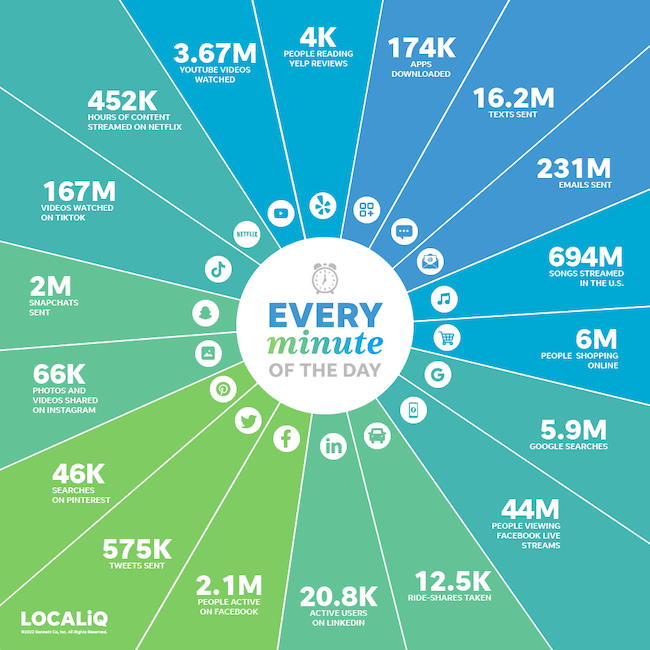
\includegraphics[scale=0.375]{internet-minute-infographic.png}
\end{frame}


%%%%%%%%%%%% 
\begin{frame}{Machine Learning vs. Econometrics}
\begin{witemize}
\item If the goal is prediction, ML methods beat econometrics (lasso, regression trees, random forests, etc.)
\item However, more data cannot solve a causal inference problem. But that's ok! 
\item Lots of applications when prediction is useful.
\begin{itemize}
\normalsize
\item Macro or financial forecasting
\item Predicting valuations for new products
\item Optimizing marketing campaigns
\item Others?
\end{itemize}
\end{witemize}
\end{frame}

\begin{frame}{Semantics}
Some language differences between statistics and ML:\\
\begin{witemize}
\item instance = data point
\item features = variables
\item learning = fitting models to data \\
\begin{itemize}
\normalsize
\item supervised learning: fit a function to a target (regression)
\item unsupervised learning: no target (density estimation), e.g., classification  
\end{itemize}
\end{witemize}
\end{frame}

%%%%%%%%%%%% 
\begin{frame}{Machine Learning}
But what about statistical inference? \\
\begin{witemize}
  \item How does the researcher know they are fitting true relationships to data and not those that have arisen spuriously from chance?
  \item Traditional null hypothesis significance testing is of limited use given millions of observations
  \item Solution: approximate out-of-sample fit using a training–validation-testing split of the underlying data
\end{witemize}
\end{frame}

%%%%%%%%%%%% 
\begin{frame}{}
\centering
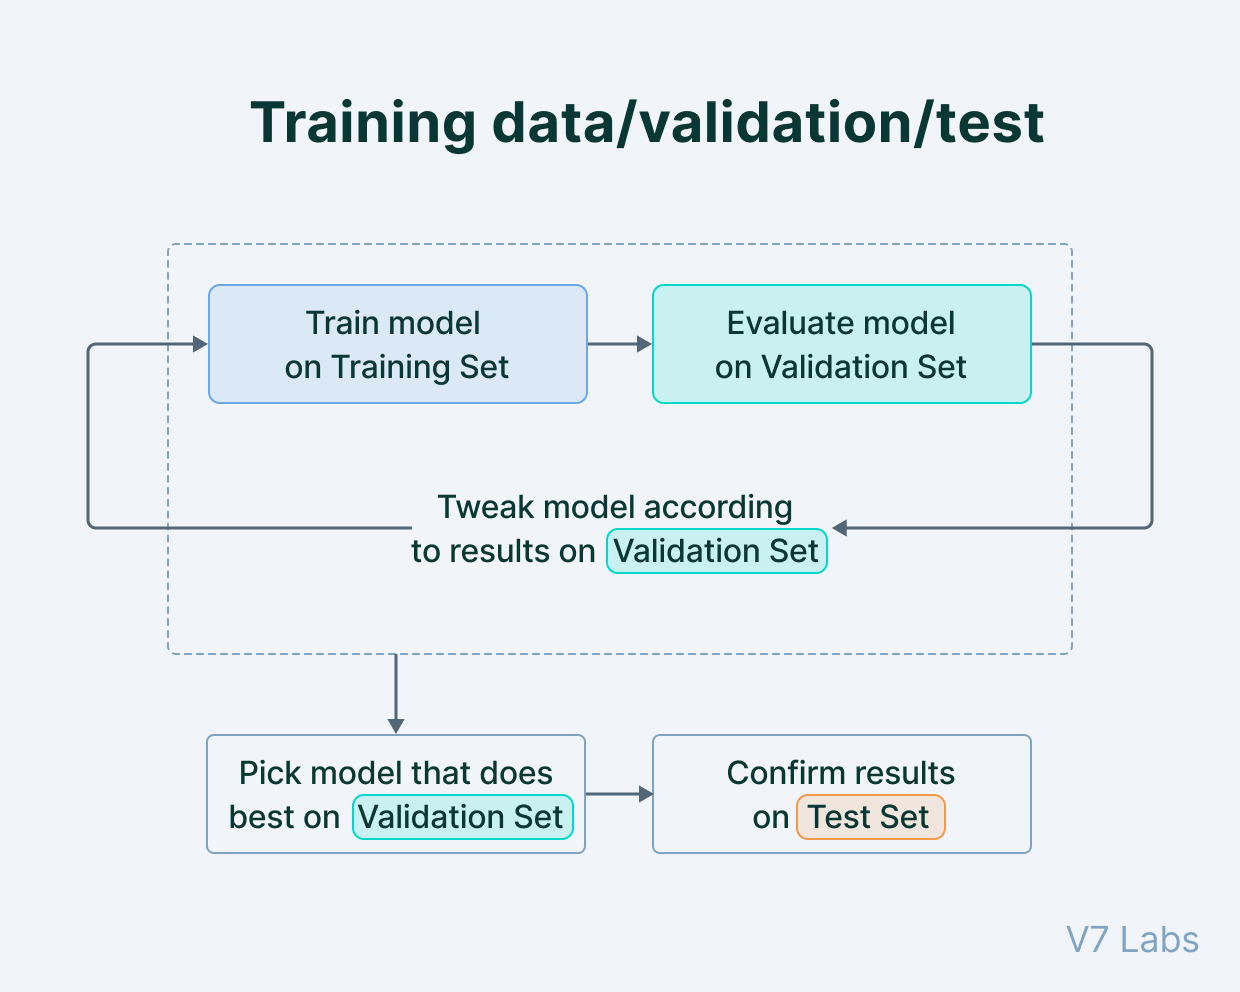
\includegraphics[scale=0.55]{61568656a13218cdde7f6166_training-data-validation-test.png}
\end{frame}

%%%%%%%%%%%% 
\begin{frame}{Example: Spam Detection}
\begin{witemize}
\item Spam Detection \\
\item[] Represent each message by features (e.g., keywords, spelling, etc.) \\~\\
\small
\begin{tabular}{cccc|c}
 ``money'' & ``Mr.'' & bad-spelling & known-sender & spam?  \\
  \hline
Y & Y & Y & N & Y \\
N & N & N & N & N \\
Y & N & Y & Y & N \\
N & Y & Y & N & Y \\
Y & N & N & N & Y \\
N & N & N & Y & N \\
\end{tabular}
\end{witemize}
Come up with rules: predict spam if... 
\end{frame}

%%%%%%%%%%%% 
\begin{frame}{An ML Algorithm: Decision Trees}
\small
With all the data, no need to fit a linear model, can be more flexible \\
\begin{center}
	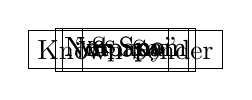
\begin{tikzpicture}[
    node/.style={%
      draw,
      rectangle,
    },
  ]
    \node [node] (A) {Known Sender };
    \path (A) ++(-135:\nodeDist) node [node] (B) {Not Spam};
    \path (A) ++(-45:\nodeDist) node [node] (C) {``money''};
    \path (C) ++(-135:\nodeDist) node [node] (D) {Spam};
    \path (C) ++(-45:\nodeDist) node [node] (E) {Not Spam};

    \draw (A) -- (B) node [left,pos=0.25] {yes}(A);
    \draw (A) -- (C) node [right,pos=0.25] {no}(A);
    \draw (C) -- (D) node [left,pos=0.25] {yes}(A);
    \draw (C) -- (E) node [right,pos=0.25] {no}(A);
\end{tikzpicture}
\end{center}
Not necessary that all variables are relevant. ML pays attention to ``feature selection.''
\end{frame}

%%%%%%%%%%%% 
\begin{frame}{Machine Learning: Other Applications}
\begin{witemize}
  \item Face detection and recognition
  \item Weather prediction
  \item Diagnosing diseases
  \item Predict whether a user will click on an add
  \item Predict stock prices 
\end{witemize}
\end{frame}

%%%%%%%%%%%% 
\begin{frame}{Artificial Intelligence and Machine Learning}
\begin{witemize}
  \item Artificial intelligence: the general ability of computers to emulate human thought and perform tasks e.g. computer games, smart speakers, etc.
  \item How can a computer play a game? \\ \pause
  \textit{Moves are determined by an algorithm, which is designed to mimic human thought processes and decision-making.}
  \item How to come up with this algorithm? \vspace{0.25em}
  \begin{itemize}
  \item Traditional AI: pre-programmed directly using human judgement
  \item Machine Learning: learn from data on past games
\end{itemize}

\end{witemize}
\end{frame}

%%%%%%%%%%%% 
\begin{frame}{Tic Tac Toe}
\begin{witemize}
  \item You can play Tic Tac Toe (and much more complex games) with a computer
  \item Computer's intelligence is pre-determined by rules like \vspace{0.25em}
  \begin{itemize}
  \item ``if the opponent has two in a row, block them,'' or 
  \item ``take the center square if it's available.''
\end{itemize}
\item These pre-programmed algorithms are ``\textit{Artificial Intelligence}''
\item One way to come up with these rules is to just pre-program them directly using human judgment
\end{witemize}
\end{frame}

%%%%%%%%%%%% 
\begin{frame}{Tic Tac Toe}
\begin{witemize}
\item Another way to teach the computer to play a game is to use Machine Learning, in which the computer learns from data on past games 
\item In this approach, the ML model identifies patterns and strategies from the game data. 
\item For example, it might notice that taking the center square often leads to a win, or that blocking an opponent's potential line of three is a good defensive strategy.
\item ML enables us to automate teaching computers to build AI 
\end{witemize}
\end{frame}

%%%%%%%%%%%% 
\begin{frame}{Natural Language Processing}
\begin{witemize}
  \item NLP: subfield of artificial intelligence (AI) and computational linguistics
  \item NLP is concerned with developing algorithms and models that allow computers to understand our language
  \item In NLP, ML is used to develop models that can learn from large amounts of text data and identify patterns and relationships in that data
  \item Uses: ChatGPT, Chatbots, translation, sentiment analysis, summarizing text
\end{witemize}
\end{frame}

%%%%%%%%%%%% 
\begin{frame}{From the Horse's Mouth}
ChatGPT on ChatGPT: \\~\\
\begin{quote}
The model is trained on a large dataset of text, and during training, it learns to predict the probability of each word in a given context based on the words that came before it. \\ \vspace{0.5em}
When answering questions, ChatGPT generates a probability distribution over all possible responses and then selects the most likely response based on that distribution. \\~\\
\end{quote}
It is truly ``Artificial'' Intelligence!
\end{frame}

%%%%%%%%%%%%%%%%%%%%
\begin{frame}{What's next}
\begin{witemize}
  \item Final research paper due today
  \item Review class this Thursday 
  \item Material for the final exam uploaded on the Course Website
  \item Final exam from 1--2.50 pm on Thursday 
  %\item Please fill the SOQs :)
\end{witemize}

\end{frame}


\end{document}